\chapter{Arquitecturas ILP}
Este capítulo trata sobre arquitecturas con paralelismo a nivel de instrucción (\emph{Instruction Level Parallelism}, ILP). Comentaremos una de las formas de incrementar el número de instrucciones por ciclo (IPC) en un procesador segmentado, que consiste en incrementar el número de instrucciones que se emiten a las unidades funcionales donde se ejecutan las operaciones que las instrucciones codifican.

Esta funcionalidad es perseguida tanto por procesadores superescalares como por procesadores VLIW, cuyas diferencias comenzaremos a destacar.

\section{Introducción}

\subsubsection{Nomenclatura}
Históricamente se utilizaba ``arquitectura de un computador'' para hacer referencia al repertorio de instrucciones que implementaba su procesador. Sin embargo, se comenzó a usar la palabra ``microarquitectura'' para ello, dejando la palabra ``arquitectura'' para denotar cómo está implementada la microarquitectura: qué unidades tiene, cómo están comunicadas entre sí, cómo funciona cada una, \ldots\\

A lo largo de esta sección hablaremos largo y tendido sobre cómo se ejecutan las instrucciones. Para ello, convenimos en decir que:
\begin{itemize}
    \item Una instrucción se está \underline{procesando} cuando está en alguna etapa del cauce de procesamiento de la misma.
    \item Una instrucción se está \underline{ejecutando} cuando está en la etapa de ejecución del cauce de procesamiento.
\end{itemize}
Finalmente, aconsejamos consultar la Sección~\ref{subsec:repaso_ILP}, antes de continuar con la lectura de este capítulo.

\subsection{Diferencias entre núcleos ILP}\label{sec:diff_ilp}
En los núcleos que implementan paralelismo a nivel de instrucción (aquellos que son capaces de emitir más de una instrucción por ciclo), nos encontramos con dos grandes familias:
\begin{description}
    \item [Núcleos ILP superescalares.]~\\
        Replican alguna de las unidades funcionales del cauce de procesamiento de instrucciones. 

        De esta forma, es el hardware quien se encarga de la planificación de las instrucciones (decide qué instrucciones se emitirán a la vez en cada momento).
    \item [Núcleos ILP con VLIW.]~\\
        Donde VLIW significa \emph{Very Long Instruction Word}, estos procesadores realmente sólo emiten una instrucción por ciclo, pero cada una de ellas codifica varias operaciones (cada una correspondería a una instrucción en arquitecturas escalares). 

        Por tanto, no hay hardware que se encargue de la planificación de instrucciones, sino que es el software (los compiladores) quien se encarga de la planificación de instrucciones, generando instrucciones largas que contienen las operaciones que se emitirán juntas durante la ejecución.
\end{description}
Las dos implementaciones segmentan el procesamiento de las instrucciones en etapas, que se corresponden con las de la Sección~\ref{subsec:repaso_ILP}.\\

Debido al menor uso de hardware que requieren los núcleos VLIW, suelen usarse en computadores empotrados.\\

\section{Microarquitectura de ILP superescalares}
Las instrucciones se captan según el orden del programa, que pasan al buffer de instrucciones, donde esperan a decodificrase en este mismo orden. Una vez decodificada la instrucción, ya se saben los recursos a utilizar por la misma, por lo que pasa a la fase de emisión.

La emisión a ejecución puede realizarse con el orden del programa o de forma desordenada, con el fin de ahorrar tiempos de ejecución (suele hacerse lo segundo). Ya sea ordenada o no, como cada instrucción supone un tiempo distinto, la finalización de las instrucciones será desordenada. Esto es, podemos tener una instrucción que pase antes a ejecución y que termine después que una instrucción que entró después a ejecución, ya que esta segunda era mucho más corta que la primera.\\

En los superescalares, la última etapa del cauce de procesamiento de instrucciones (dedicada a \emph{write-back}) procesa las mismas de forma ordenada (según el orden del programa), a pesar de que se produzca una ejecución desordenada de las instrucciones.

Con esto, se garantiza la consistencia del procesador, de forma que el resultado tras ejecutar una serie de instrucciones coincida con el que provocaría la ejecución ordenada de las mismas.\\

La realidad es que cada una de las etapas desarrolladas en la Sección~\ref{subsec:repaso_ILP} se dividen a su vez en subetapas. Podemos encontrar implementaciones que realicen hasta 14 subetapas en las etapas más complejas.

\subsubsection{Dependencias y riesgos}
La segmentación nos permite disminuir el tiempo de ciclo de la CPU, reduciéndolo hasta en $N$ veces el tiempo de ciclo anterior, siendo $N$ el número de etapas del cauce (suponiendo que todas las etapas duran lo mismo).

Sin embargo, en los códigos a ejecutar nos encontramos con dependencias (de datos, de control o estructurales) que dan lugar a problemas en el cauce segmentado, los cuales pueden conducir a los programas a un resultado incorrecto en su ejecución. Todos estos problemas reciben el nombre de \emph{hazards} (o riesgos).\\

Para eliminar riesgos en los núcleos VLIW se deben introducir operaciones de no operación (\verb|nop|). Esto provoca una disminución en las prestaciones del núcleo (al desperdiciar ciclos de instrucción). Esta disminuición de las prestaciones es aún peor en los procesadores VLIW superescalares (núcleos capaces de dar por un ciclo varias instrucciones VLIW), donde obtenemos un IPC mucho mayor al introducir operaciones \verb|nop| que los que ya obteníamos en el VLIW escalar.

Todo esto sin considerar las dependencias estructurales (las cuales se detectan cuando en tiempo de ejecución dos instrucciones tratan de acceder a la misma unidad funcional), lo que ralentiza aún más los tiempos de ejecución.\\

A continuación, vamos a ver cómo en los computadores ILP superescalares es el hardware quien se encarga de eliminar los riesgos y de reducir el tiempo de penalización que suponen las dependencias, pudiendo llegar a un tiempo de ejecución próximo al ideal.

\subsection{Características del cauce de instrucciones}
Desarrollamos a continuación varios aspectos relevantes del cauce de procesamiento de instrucciones a tener en cuenta, los cuales \textbf{no han sido comentados en ninguna asignatura} hasta el momento. Podemos observar un cauce real en la Figura~\ref{fig:Cauce_ARM_cortex_a76}, donde la etapa de captación es la que se marca como \emph{Front End}, en color amarillo pastel; la etapa de decodificación y emisión la de color verde pastel; la de ejecución en verde oscuro y el \emph{write-back} en lila.

\begin{figure}
    \centering
    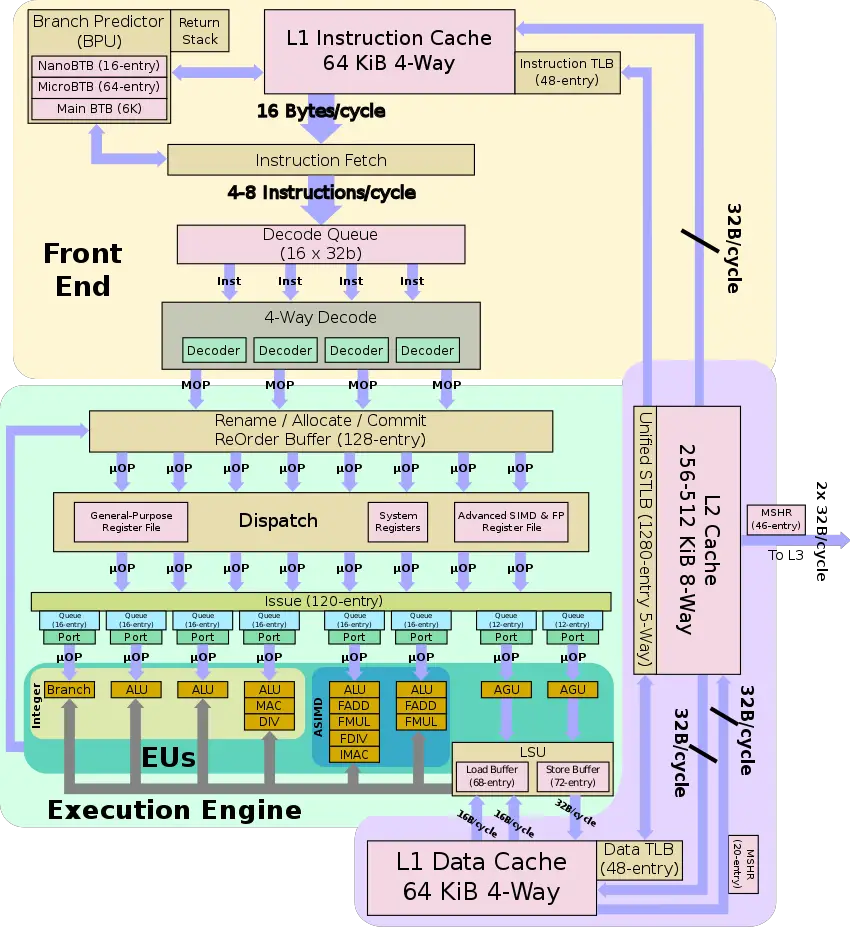
\includegraphics[width=0.8\linewidth]{Images/Cauce1.png}
    \caption{Cauce del procesador ARM cortex A76.}
    \label{fig:Cauce_ARM_cortex_a76}
\end{figure}

\begin{itemize}
    \item Como ya se comentaba en la Sección~\ref{subsec:repaso_ILP}, la etapa de ejecución y de memoria se consideraba una sola, al ser las instrucciones bien de acceso a memoria o bien instrucciones aritmético-lógicas.
    \item La etapa de emisión (aquella en la que ya se conocen los operandos y se prepara para mandar a ejecución) forma parte de la decodificación.
    \item Observamos que en la etapa amarillo pastel encontramos entre cada módulo y el siguiente 4 flechas representando puentes de datos, los cuales pasan a 8 en la etapa verde pastel. Esto sucede siempre en los x86 (son computadores CISC): sucede cuando una instrucción está implementada mediante varias microinstrucciones.
    \item En la etapa de emisión hay dos partes importantes:
        \begin{itemize}
            \item Una en la que las instrucciones son almacenadas para su ejecución en lo que se llaman estaciones de reserva (o ventana de instrucciones en el caso de Intel), mientras que la operación no está lista para pasar a su ejecución las unidades funcionales.
            \item Una en la que se mandan a la primera unidad funcional desde las estaciones de reserva.
        \end{itemize}
        Depende de la implementación del procesador, pero normalmente cada unidad funcional tiene sus propias estaciones de reserva. Podemos observarlas en la Figura~\ref{fig:Cauce_ARM_cortex_a76}, las cajas de color azul claro etiquetadas con ``Queue'' antes de las unidades funcionales de la etapa de ejecución.
    \item En relación al punto anterior, Intel llama \textbf{emisión} a ventana de instrucciones y \textbf{envío} a unidades funcionales; mientras que manuales de ARM enuncian \textbf{envío} a estaciones de reserva y \textbf{emisión} a unidades funcionales.
    \item En la Figura~\ref{fig:Cauce_ARM_cortex_a76}, destacamos las unidades de \verb|AGU| y \verb|LSU|, que son las últimas a las que van a parar las instrucciones de acceso a memoria.
        \begin{itemize}
            \item Las \verb|AGU| son unidades de cálculo arimético que se encargan de calcular direcciones de acceso a memoria, la generación del address de una instrucción de acceso a memoria\footnote{Esta es la unidad que se encarga de procesar las instrucciones leaq de ASM, que se vieron en EC.}.
            \item Las \verb|LSU| son colas FIFO en las que esperan las instrucciones de acceso a memoria. Hay una cola dedicada a las instrucciones de lectura y otra a las de escritura. 
        \end{itemize}
    La implementación de adelantamiento de lecturas a escrituras propias (que vimos en el Capítulo~\ref{chapter:Tema3} que todos los procesadores incumplían en cuanto a orden global) se implementa en estas colas LSU\@. El protocolo genérico y más sencillo para realizarlo es el siguiente.

    Si viene una nueva instrucción y es de escritura, se introduce en su cola correspondiente. Si es de lectura, tenemos dos posibilidades:
    \begin{itemize}
        \item Si el cerebro de la \verb|LSU| no encuentra ninguna escritura con la misma dirección de memeoria en la cola de escrituras, simplemente se introduce en la cola correspondiente para lecturas.
        \item Si el cerebro de la \verb|LSU| detecta al menos una escritura a la última posición de memoria, coge el contenido de la última y se lo devuelve como resultado a la instrucción de lectura, sin llegar a leer dicha instrucción de memoria, al nunca introducirse en la cola.
    \end{itemize}
    Si los \verb|LSU| funcionan al igual que una cola FIFO (puede llevar quizás implementaciones más complejas, como sucede en los ARM), entonces los órdenes $W\rightarrow W$ y $R\rightarrow R$ son garantizados por el procesador (esto es lo que sucede en los Intel).

    Cabe destacar que la velocidad de las dos colas \verb|LSU| no es la misma, al avanzar las lecturas de forma más rápida que las escrituras.
\end{itemize}

\subsubsection{Unidades de cada etapa}

\begin{figure}
    \centering
    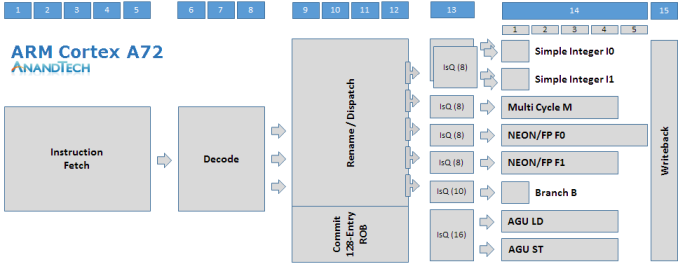
\includegraphics[width=0.8\linewidth]{Images/Cauce2.png}
    \caption{Cauce del procesador ARM cortex A72 de forma abstracta.}
    \label{fig:Cauce_ARM_cortex_a72}
\end{figure}

A continuación, en la Figura~\ref{fig:Cauce_ARM_cortex_a72} podemos volver a observar el cauce de instrucciones, esta vez de otro procesador similar, pero de una forma un tanto más abstracta. Procedemos a explicar qué unidades funcionales se encargan de realizar cada etapa, así como de explicar las funcionalidades y buffers de cada una, las cuales se desarrollarán en profundidad a lo largo del capítulo.

\begin{description}
    \item [Etapa de captación.] Formada por la unidad funcional etiquetada por ``Instruction Fetch'', recibe las instrucciones de la memoria caché L1 de instrucciones.

        Se encarga de detectar saltos y predecir saltos condicionales. Almacena la Tabla de saltos.
    \item [Etapa de decodificación y emisión.] Formada por las unidades funcionales de las columnas 6 a 12, recibe las instrucciones del IB (\emph{Instruction Buffer}), que sirve de puente entre la etapa de captación y esta.

        Se encarga primero de decodificar las instrucciones y luego de prepararlas para emisión (para enviarlas a las unidades funcionales), durante la cual (se desarrollarán pŕoximamente):
        \begin{itemize}
            \item Elimina riesgos WAW y WAR (renombrando registros con el buffer de renombrado).
            \item Elimina riesgos RAW y estructurales (mediante las estaciones de reserva).
            \item Reduce los riesgos de control (eejcución especulativa usando ROB).
            \item Captura de operandos desde registros de la arquitectura, o desde registros de renombrado.
        \end{itemize}
        Cuenta con la ventana de instrucciones o estación de reserva (las unidades de la columna 13, que preceden a la etapa de ejecución), con el Buffer de renombrado y con el Buffer de reorden (\emph{ReOrder Buffer} o ROB), que permite eliminar los riegos de control de forma sencilla. En el bloque de ``Rename/Dispatch'' tiene acceso a los registros de la arquitectura.
    \item [Etapa de ejecución.] Formada por todas las unidades de la columna 14, recibe las instrucciones de las ventanas de instrucciones o estaciones de reserva.
    \item [Etapa para \emph{write-barck}.] Formada por la unidad de la columna 15, implementa la consistencia secuencial del procesador así como la ejecución especulativa. Cuenta con un buffer de renombrado así como con el buffer de reorden (ROB).

        Además, elimina los riesgos de control que no fueron detectados por predicciones incorrectas (para ello usamos el ROB).

        Tiene acceso a los registros de la arquitectura.
\end{description}

A continuación, desarrollaremos en profundidad cómo funciona la etapa de emisión. Para ello, será necesario entender bien los buffers de renombrado, reorden y las estaciones de reserva, que son la parte principal de la etapa. Por simplicidad, en esta sección siempre que nos referimos a instrucciones, estaremos hablando de instrucciones aritméticas, que son las más completas para describir bien ambos buffers (por tener siempre un registro donde almacenar el resultado y uno o dos operandos).

\subsection{Buffer de renombrado}
Cada vez que se emite una instrucción, se le asigna una entrada en la estación de reserva, y se renombra el registro en el que se va a guardar la salida de la instrucción (siempre se renombra), asignándole una entrada en el banco de registros de renombrado (cada una de estas entradas recibirá el nombre de ``registro de renombrado'').

\begin{description}
    \item [Entrada válida.] Bit que indica si la entrada de la tabla está en uso o no.
    \item [Registro de destino.] Se indica el registro que está siendo renombrado (un 3 en la entrada 5ª indica que el registro de renombrado número 5 está renombrando al registro número 3).

        Próximamente, nos referiremos por \verb|Ri| al registro número $i$, y por \verb|RRi| al registro de renombrado número $i$.
    \item [Valor.] Se almacena el valor que contendría el registro.
    \item [Valor válido.] Un bit que indica si el valor de la columna anterior es válido (esto es, que ha sido ya calculado), o no (la instrucción que da el valor fue emitida pero no terminó).
    \item [Último.] Un bit que indica que es el último renombrado de un registro. Sólo puede estar activo en una única entrada, por cada registro de renombrado que renombre a un mismo registro.

        Por ejemplo, si el registro número 5 está siendo renombrado varias veces por varios registros de renombrado, la entrada que contenga un 1 en esta columna contendrá el valor válido para dicho registro.
\end{description}
A la hora de captar operandos, si necesitamos por ejemplo obtener el valor del registro 5: 
\begin{itemize}
    \item Si este se encuentra renombrado (es decir, fue usado para almacenar el valor resultante de una operación), se captará el valor del buffer de renombrado del registro de renombrado con el campo ``Último'' a 1 (en caso de que tenga el bit de ``Valor válido'' a 1, si no esperará a que esté listo el dato).
    \item En caso contrario, se capta directamente del registro número 5.
\end{itemize}

Al renombrar siempre el registro que almacena el resultado de una instrucción, nunca podrán producirse dependencias de tipo WAW y WAR (eliminamos dichas depedencias), por lo que no es necesario detectarlas.

\begin{ejemplo}\label{ejm:T4_1}
    Supongamos que queremos ejecutar el siguiente código en el procesador, en el que las instrucciones se emiten de forma secuencial:
    \begin{listing}[H]
    \begin{minted}[xleftmargin=6cm, linenos]{c++}
R3 = R3 - R5
R4 = R3 + 1
R3 = R5 + 1
R7 = R3 * R4
    \end{minted}
    \caption{Código a ejecutar}
    \label{cod:ejm1_T4}
    \end{listing}
    Donde ningún registro ha sido renombrado todavía salvo el registro \verb|R5|, cuya entrada en el buffer de renombrado observamos en la Tabla~\ref{tab:ejm1_T4}. El registro 3 tiene como valor inicial 62.
    \begin{table}[H]
    \centering
    \begin{tabular}{|c|c|c|c|c|c|}
        \hline
        Nº entrada & EV & Registro & Valor & Válido & Último \\
        \hline
        0 & 1 & 5 & 58 & 1 & 1 \\
        \hline
    \end{tabular}
    \caption{Estado inicial del buffer de renombrado}
    \label{tab:ejm1_T4}
    \end{table}
    Así pues, el buffer de renombrado tras la ejecución de nuestro programa de 4 líneas será el que podemos observar en la Tabla~\ref{tab:ejm1_T4_2}. Describimos los pasos que nos han llevado a obtener dicho estado en el buffer:
    \begin{itemize}
        \item Línea 1: Creamos una entrada para el registro 3, no completando el campo de valor (ya que la instrucción todavía no terminó de ejecutarse), luego con un 0 en válido y un 1 en último (es el último renombramiento del registro 3).
        \item Línea 2: Creamos una entrada para el registro 4, no completando el campo de valor, luego con un 0 en válido y un 1 en último.
        \item Línea 3: Creamos una entrada para el registro 3, no completando el campo de valor, luego con un 0 en válido y un 1 en último. Además, el 1 del último de la última vez que renombramos el registro 3 pasa a valer 0.
        \item Línea 4: Creamos una entrada para el registro 7, no completando el campo de valor, luego con un 0 en válido y un 1 en último.
    \end{itemize}
    Cuando se vayan completando las ejecuciones de las instrucciones (la etapa de ejecución), se actualizará en cada entrada el valor y, posteriormente, se cambiará la columna de válido a 1. La Tabla~\ref{tab:ejm1_T4_2} muestra que las instrucciones 1 y 2 se completaron pero que la 3 y 4 todavía no.
    \begin{table}[H]
    \centering
    \begin{tabular}{|c|c|c|c|c|c|}
        \hline
        Nº entrada & EV & Registro & Valor & Válido & Último \\
        \hline
        0 & 1 & 5 & 58 & 1 & 1 \\
        \hline
        1 & 1 & 3 & 4 & 1 & 0 \\
        \hline
        2 & 1 & 4 & 5 & 1 & 1 \\
        \hline
        3 & 1 & 3 &   & 0 & 1 \\
        \hline
        4 & 1 & 7 &   & 0 & 1 \\
        \hline
    \end{tabular}
    \caption{Estado del buffer de renombrado}
    \label{tab:ejm1_T4_2}
    \end{table}
    Tras este renombramiento, el Código~\ref{cod:ejm1_T4} pasaría a ser para el procesador (notando por \verb|RR| a los registros de renombrado) el que muestra el Código~\ref{cod:ejm1_T4_2}, que ya no tiene las dependencias WAW y WAR que tenía el anterior Código~\ref{cod:ejm1_T4} (una dependencia WAW entre las líneas 1 y 3, y una WAR entre las líneas 2 y 3). Sin embargo, observamos que siguen existiendo dependencias RAW (entre las líneas 1 y 2), las cuales se eliminarán con el uso de las estaciones de reserva.
    \begin{listing}[H]
    \begin{minted}[xleftmargin=6cm, linenos]{c++}
RR1 = R3 - RR0        
RR2 = RR1 + 1
RR3 = RR0 + 1
RR4 = RR3 * RR2
    \end{minted}
    \caption{Código ejecutado por el procesador}
    \label{cod:ejm1_T4_2}
    \end{listing}
\end{ejemplo}

\subsection{Estaciones de reserva}
Cada unidad funcional tiene sus propias estaciones de reserva, tal y como puede observarse en la Figura~\ref{fig:Cauce_ARM_cortex_a72} (en la columna 13). Por ejemplo, la estación de reserva de la unidad para multiplicaciones suele ser independiente de la estación de reserva para la unidad de sumas y restas. 

Una estación de reserva es una tabla donde se almacenan las instrucciones que todavía no han sido emitidas a unidades funcionales. La razón por la que estén en estas estaciones puede ser o bien que estén esperando a un operando que está siendo calculado, o bien que la unidad funcional a la que van a entrar está siendo usada por otra instrucción.

Los campos de una tabla de estación de reserva son los siguientes:
\begin{description}
    \item [Código de operación.] Se guarda la instrucción que no ha sido emitida todavía. Por ejemplo: \verb|add|, \verb|mult|, \ldots
    \item [Registro de destino.] Se guarda el registro de renombrado en el que almacenar el resultado de la instrucción cuando esta finalice.
    \item [Operando i-ésimo.] Se guarda el operando i-ésimo para la instrucción, o el registro de renombrado de donde obtener el operando cuando termine de calcularse.
    \item [OK i-ésimo.] Bit que controla la columna anterior:
        \begin{itemize}
            \item Si contiene un 1, indica que el operando i-ésimo es el valor que se encuentra en la columna anterior. 

                Indica que el operando está listo para su uso.
            \item Si contiene un 0, indica que el operando i-ésimo va a ser obtenido del registro de renombrado número la columna anterior, cuando este termine de calcularse. 

                Indica que se está esperando al operando.
        \end{itemize}
\end{description}
Lo normal es que una instrucción tenga dos operandos (1 y 2).\\

Cuando una instrucción pasa a la fase de emisión, se genera una entrada en la estación de reserva para la misma. En esta se rellena el campo de código de operación, registro de destino y:
\begin{itemize}
    \item Si un operando se sabe ya, se introduce en el campo correspondiente, pondiendo el campo de OK correspondiente a 1.
    \item Si se está calculando todavía, se pone el campo OK correspondiente a 0 y se indica la entrada del registro de renombrado de la que se captará el valor una vez esté listo.
\end{itemize}
Cuando una unidad funcional termina el cálculo de un dato, este pasa al bus de salida de la unidad, con un paquete que contiene el registro de renombrado en el que se escribirá junto con el valor a escribir. El paquete es recibido por el registro de renombrado correspondiente, que escribe el valor y cambia el bit del campo ``Valor válido'' a 1.

Además, las estaciones de reserva se encuentran espiando dicho bus, para que cuando se vaya a escribir en un registro de renombrado que se encuentra en una entrada como operando no válido, la estación de reserva capte su valor, cambiando ahora el bit de ``OK'' a 1, y teniendo ahora el operando disponible.\\

Cuando una entrada de la tabla de la estación de reserva está completa (dispone de todos los operandos), pasará a ejecución en el siguiente ciclo (en caso de tener la unidad funcional correspondiente libre, evitando también riesgos estructurales). De esta forma, se eliminan las dependencias de tipo RAW (por lo que no será necesario su detección y eliminación, al hacerlo este proceso de forma automática).

Se pueden enviar instrucciones a emisión de forma paralela.\\

El algoritmo realizado de forma simultánea por el buffer de renombrado y las estaciones de reserva es el \textbf{algoritmo de Tomasulo}.

A continuación, mostramos un par de ejemplos para familiarizarnos con el uso de las estaciones de reserva.

\begin{ejemplo}
    Queremos ejecutar el Código ensamblador~\ref{cod:ejm2_T4} (donde suponemos que el primer registro es el destino) en un procesador con una estación de reserva centralizada, que suponemos que sólo emite una instrucción por ciclo y además lo hace de forma ordenada. Mostrar cómo van cambiando las tablas del buffer de renombrado y de la estación de reserva. El estado inicial del banco de registros es el que se observa en la Tabla~\ref{tab:ejm2_T4_registros}.\\
    \begin{listing}[H]
    \begin{minted}[xleftmargin=6cm, linenos]{c++}
mult r2, r0, r1        
add  r3, r1, r2
sub  r2, r0, r1
    \end{minted}
    \caption{Código a ejecutar}
    \label{cod:ejm2_T4}
    \end{listing}

    \begin{table}
    \centering
    \begin{tabular}{|c|c|c|c|c|c|}
        \hline
        \verb|r0| & \verb|r1| & \verb|r2| & \verb|r3| & \verb|r4| & \verb|r5| \\ 
        \hline
        0 & 10 & 20 & 30 & 40 & 50 \\
        \hline
    \end{tabular}
    \caption{Estado inicial de los registros}
    \label{tab:ejm2_T4_registros}
    \end{table}

    A continuación, describimos las accesiones que realiza el procesador en el proceso de emisión, mostrando finalmente las Tablas~\ref{tab:ejm2_T4_renombrado} y~\ref{tab:ejm2_T4_estacion}, que contienen respectivamente el estado final del buffer de renombrado y de la estación de reserva (en estas, no borramos lo que había antes, sino que lo tachamos para que puedan verse los diferentes estados por los que han pasado los campos).
    \begin{enumerate}
        \item La instrucción 1 llega a emisión, con lo que se abre un campo en la estación de reserva para la misma, así como un campo en el buffer de renombrado, por ser una intrucción aritmético-lógica (tiene salida a un registro). Esto no se comentará en las siguientes instrucciones.

            En el buffer de renombrado se introduce como registro el 2, que todavía no tiene un valor.

            En la estación de reserva se introduce la operación, con el registro de renombrado destino el número 0 (ya que pusimos la entrada 0 como renombrado del registro 2).

            La instrucción pasará en el siguiente ciclo a ejecución, por estar su unidad funcional libre y disponer de todos los operandos.
        \item En el buffer de renombrado se introduce como registro el 3, que tampoco tiene un valor.

            En la estación de reserva se introduce la operación, con el registro de renombrado destino el 1.

            A la instrucción le falta el 2o operando, por lo que tendrá que esperar a la finalización de la instrucción 1.
        \item En el buffer de renombrado se introduce como registro el 2, cambiando el 1 del campo ``Último''  de la entrada 0 a 0.

            En la estación de reserva se introduce la operación, con el registro de renombrado destino el 2.

            A la instrucción no le faltan operandos, pero debe emitirse en orden del programa\footnote{Nos lo dice el enunciado.} por lo que debe ejecutarse antes la operación \verb|add| para poder ejecutarse esta.
        \item Suponemos que ahora termina la instrucción \verb|mult|, con lo que se modifican los campos ``Valor'' y ``Válido'' del buffer de renombrado, con el valor final de la operación. 

            La estación de reserva observa dicha modificación y, como tenía en operando 2 el registro de renombrado 0 como registro de donde obtener el operando, obtiene el resultado, siendo ahora válido el operando, con lo que pasará a ejecución en el siguiente ciclo.
        \item Suponemos que termina la instrucción 2, luego completará los valores en el buffer de renombrado y pasará a ejecución la instrucción 3.
        \item La instrucción 3 terminará su ejecución y completará los valores en el buffer de renombrado.
    \end{enumerate}

    \begin{table}[H]
    \centering
    \begin{tabular}{|c|c|c|c|c|c|}
        \hline
        Nº entrada & EV & Registro & Valor & Válido & Último \\
        \hline
        0 & 1 & 2 & \bcancel{-}\ 0 & \bcancel{0}\ 1 & \bcancel{1}\ 0 \\
        \hline
        1 & 1 & 3 & \bcancel{-}\ 10 & \bcancel{0}\ 1 & 1 \\
        \hline
        2 & 1 & 2 & \bcancel{-}\ -10 & \bcancel{0}\ 1 & 1 \\
        \hline
    \end{tabular}
    \caption{Estado final del buffer de renombrado}
    \label{tab:ejm2_T4_renombrado}
    \end{table}

    \begin{table}[H]
    \centering
    \begin{tabular}{|c|c|c|c|c|c|}
        \hline
        Cod. Op. & Destino & Op. 1 & OK 1 & Op. 2 & OK 2 \\
        \hline
        \verb|mult| & 0 & 0 & 1 & 10 & 1 \\
        \hline
        \verb|add| & 1 & 10 & 1 & \bcancel{0}\ 0 & \bcancel{0}\ 1 \\
        \hline
        \verb|sub| & 2 & 0 & 1 & 10 & 1 \\
        \hline
    \end{tabular}
    \caption{Estado final de la estación de reserva}
    \label{tab:ejm2_T4_estacion}
    \end{table}

    De esta forma, vemos que el código ejecutado fue realmente el Código~\ref{cod:ejm2_T4_final}.
    \begin{listing}[H]
    \begin{minted}[xleftmargin=6cm, linenos]{c++}
RR0 = R0 * R1
RR1 = R1 + RR0
RR2 = R0 - R1
    \end{minted}
    \caption{Código ejecutado realmente}
    \label{cod:ejm2_T4_final}
    \end{listing}
\end{ejemplo}

Repetimos el ejemplo de la Sección~\ref{ejm:T4_1}, ahora viendo cómo evoluciona la tabla de la estación de reserva (suponiendo que se usa la misma para todas las unidades funcionales).

\begin{ejemplo}
    Supongamos que queremos ejecutar el Código~\ref{cod:ejm1_T4} en el procesador, donde ningún registro ha sido renombrado todavía salvo el registro \verb|R5|, cuya entrada en el buffer de renombrado observamos en la Tabla~\ref{tab:ejm1_T4}. El registro 3 tiene como valor inicial 62.

    Ahora, no comentaremos las acciones realizadas, simplemente mostramos el estado final del buffer de renombrado, en la Tabla~\ref{tab:ejm3_T4_renombrado}; así como el estado final de la tabla de la estación de reserva, en la Tabla~\ref{tab:ejm3_T4_estacion}. En vez de borrar los estados intermedios los tachamos, para que quede constancia de ellos.

    Hemos considerado que primero se meten todas las instrucciones y luego se completa la primera, para mayor simplicidad.\\

    \begin{table}[H]
    \centering
    \begin{tabular}{|c|c|c|c|c|c|}
        \hline
        Nº entrada & EV & Registro & Valor & Válido & Último \\
        \hline
        0 & 1 & 5 & 58 & 1 & 1 \\
        \hline
        1 & 1 & 3 & \bcancel{-}\ 4 & \bcancel{0}\ 1 & \bcancel{1}\ 0 \\
        \hline
        2 & 1 & 4 & \bcancel{-}\ 5 & \bcancel{0}\ 1 & 1 \\
        \hline
        3 & 1 & 3 & \bcancel{-}\ 59 & \bcancel{0}\ 1 & 1 \\
        \hline
        4 & 1 & 7 & \bcancel{-}\ 295 & \bcancel{0}\ 1 & 1 \\
        \hline
    \end{tabular}
    \caption{Estado final del buffer de renombrado}
    \label{tab:ejm3_T4_renombrado}
    \end{table}

    \begin{table}[H]
    \centering
    \begin{tabular}{|c|c|c|c|c|c|}
        \hline
        Cod. Op. & Destino & Op. 1 & OK 1 & Op. 2 & OK 2 \\
        \hline
        \verb|sub| & 1 & 62 & 1 & 58 & 1 \\
        \hline
        \verb|add| & 2 & \bcancel{1}\ 4 & \bcancel{0}\ 1 & 1 & 1 \\
        \hline
        \verb|add| & 3 & 58 & 1 & 1 & 1 \\
        \hline
        \verb|mult| & 4 & \bcancel{3}\ 59 & \bcancel{0}\ 1 & \bcancel{2}\ 5 & \bcancel{0}\ 1 \\
        \hline
    \end{tabular}
    \caption{Estado final de la estación de reserva}
    \label{tab:ejm3_T4_estacion}
    \end{table}

    De esta forma, el código que se ejecutó en el procesador fue el Código~\ref{cod:ejm3_T4_final}.
    \begin{listing}[H]
    \begin{minted}[xleftmargin=6cm, linenos]{c++}
RR1 = R3 - RR0
RR2 = RR1 + 1
RR3 = RR0 + 1
RR4 = RR3 * RR2
    \end{minted}
    \caption{Código ejecutado}
    \label{cod:ejm3_T4_final}
    \end{listing}
\end{ejemplo}

\subsection{Buffer de reorden, ROB}
En la etapa de \emph{write-back}, se pasarán los valores de los registros de renombre a los registros de la arquitectura, siguiendo el orden del programa.

Para ello, será necesario disponer de un buffer de reorden (\emph{ReOrder Buffer}, ROB), el cual permite modificar los registros de la arquitectura en orden del programa, así como implementar de una forma muy sencilla la ejecución especulativa, la cual nos reduce los riesgos de control de una forma muy sencilla.

\subsubsection{Ejecución especulativa}
La ejecución especulativa es el proceso mediante el cual el procesador predice el resultado de un salto (supone que se realizará, o que no) y actúa en consecuencia a ello. Cuando se sepa de verdad si el salto se realiza o no:
\begin{itemize}
    \item Si el procesador predijo bien el salto, habrá eliminado la latencia introducida por el riesgo de control de dicho salto.
    \item Si no lo predijo bien, el procesador debe eliminar los cálculos hechos y comenzar a realizar los cálculos correctos.
\end{itemize}
Ilustramos la funcionalidad de la ejecución especulativa con el siguiente ejemplo:
\begin{ejemplo}
    Suponamos que disponemos del Código~\ref{cod:ejm4_T4}:
    \begin{listing}[H]
    \begin{minted}[xleftmargin=6cm]{c++}
if (a < b){
    // Bloque A
}else{
    // Bloque B
}
    \end{minted}
    \caption{Código del programa}
    \label{cod:ejm4_T4}
    \end{listing}
    el cual se implementa en ensamblador mediante saltos. Supongamos que ante el primer salto la predicción del procesador es que se saltará. Entonces, las siguientes instrucciones a ejecutar serán las del bloque A, por lo que el procesador empieza a ejecutar dichas instrucciones \textbf{de forma especulativa} (suponiendo que se va a saltar). Cuando se conoce si se va a saltar o no (cuando la instrucción de salto termina la etapa de ejecución):
    \begin{itemize}
        \item Si se iba a saltar (la predicción acertó), se continúa con la ejecución del bloque A.
        \item Si no se iba a saltar (la predicción falló), se descartan los cálculos realizados, y se comienza a ejecutar el bloque B.
    \end{itemize}
\end{ejemplo}

Una vez conocida qué es la ejecución especulativa, pasamos ahora con otro ejemplo, que sirve de motivación para reordenar código; y de ejemplo de necesitar el ROB.

\begin{ejemplo}
    Supongamos que queremos ejecutar el Código ensamblador~\ref{cod:ejm5_T4}, que multiplica dos vectores de datos \verb|double| que comienzan en \verb|0x1C| y \verb|0x2D| respectivamente por el contenido de \verb|r6|, usando \verb|r2| como índice y \verb|r4| como número de componentes del vector:\\
    \begin{listing}[H]
    \begin{minted}[xleftmargin=2cm, linenos]{asm}
loop:   ld   r1, 0x1C(r2)     # r1 <-- M[1C + [r2]]
        mul  r1, r1, r6       # r1 <-- r1 * r6
        st   r1, 0x1C(r2)     # M[1C + [r2]] <-- r1
        ld   r3, 0x2D(r2)     # r3 <-- M[2D + [r2]]
        mul  r3, r3, r6       # r3 <-- r3 * r6
        st   r3, 0x2D(r2)     # M[2D + [r2]] <-- r3
        addi r2, r2, #1       # r2++
        subi r4, r4, #1       # r4--
        bnz  r4, loop         # Si r4 != 0, jump loop
    \end{minted}
    \caption{Código a ejecutar}
    \label{cod:ejm5_T4}
    \end{listing}

    Supongamos que tenemos 4 unidades funcionales: 
    \begin{itemize}
        \item Una para operaciones de coma flotante.
        \item Una para operaciones con enteros.
        \item Una para cargas y almacenamientos en memoria.
        \item Una para realizar saltos.
    \end{itemize}
    Estudiamos ahora cómo podemos paralelizar el código de forma que podamos aprovechar dichas unidades funcionales, extrayendo paralelismo.

    Las dependencias tipo WAR y WAW (como por ejemplo entre las líneas 6 y 7) no nos preocupan, pues el buffer de renombrado las elimina. Además, como todos los procesadores implementan el adelantamiento $W\rightarrow R$ y se tiene que $0x1C + r2 \neq 0x2D + r2$, la lectura de la línea 4 puede adelantar a la de la línea 3. 

    Aplicando estas dos mejoras, obtenemos que el código puede paralelizarse de la siguiente forma:\\
    \begin{listing}[H]
    \begin{minted}[xleftmargin=1cm]{asm}
ld  r1, 0x1C(r2)
mul r1, r1, r6      ld  r3, 0x2D(r2)
st  r1, 0x1C(r2)    mul r3, r3, r6      addi r2, r2, #1
                    st  r3, 0x2D(r2)    subi r4, r4, #1
                                        bnz  r4, loop
    \end{minted}
    \caption{Código paralelizado}
    \label{cod:ejm4_T4_paralelizado}
    \end{listing}

    Notemos que la línea 1 y 4 no pueden ejecutarse a la vez por sólo haber una unidad funcional de acceso a memoria. Así mismo, la instrucción 7 puede ejecutarse en paralelo con la 5 por operar una con enteros y otra con números de coma flotante.\\
    
    Sin embargo, si cambiamos el código de forma que las líneas 3 y 4 pasen a ser las del Código~\ref{cod:ejm4_T4_cambiarcodigo}, donde para un vector usamos el registro \verb|r2| como índice y para el otro el \verb|r7|, podría suceder que $0x1C + r2 = 0x2D + r7$, produciéndose una dependencia de tipo RAW y no pudiendo ejecutar el código en paralelo.
    \begin{listing}[H]
    \begin{minted}[xleftmargin=6cm]{asm}
st  r1, 0x1C(r2)
ld  r3, 0x2D(r7)
    \end{minted}
    \caption{Cambiamos dos instrucciones}
    \label{cod:ejm4_T4_cambiarcodigo}
    \end{listing}
    Sin embargo, para ello tenemos la carga especulativa: ejecutamos el código en paralelo como en~\ref{cod:ejm4_T4_paralelizado} de forma especulativa, suponiendo que las direcciones son distintas. Si en alguna ejecución las direcciones coinciden (esto se detecta al realizar la instrucción 3), las instrucciones que se han ejecutado entre la instrucción 1 y la 3 deben marcarse de alguna forma para que cuando pasen por la última etapa (la de \emph{write-back}) no modifiquen los registros de la arquitectura, sino que se descarten. Esta labor la realiza el ROB\@. Cuando se produzca este caso, el contador de programa debe volver a la instrucción 4, para volver a ejecutar dicha instrucción y todas las que hay detrás.
\end{ejemplo}

\subsubsection{Buffer de reorden}
El buffer de reorden (o ROB), consta de una tabla que funciona a modo de cola\footnote{Se explicará próximamente.}. Por cada instrucción que se emite, se crea una entrada en el ROB para almacenar dicha instrucción (en el orden del programa).

Cada uno de los campos del ROB se describen a continuación.
\begin{description}
    \item [Código de operación.] Se guarda el tipo de instrucción.
    \item [Número de instrucción.] Se guarda la posición de la instrucción en el código (podemos notarlo como instrucción 1, 2, \ldots o como \verb|inicio+1|, \verb|inicio+2|, \ldots).
    \item [Unidad.] Indica la unidad funcional a la que se enviará la instrucción.
    \item [Marca.] Indica el estado de la instrucción. Puede tomar los valores:
        \begin{description}
            \item [x] Para indicar que se está ejecutando.
            \item [i] Para indicar que ha sido emitida pero que no se está ejecutando.
            \item [f] Para indicar que ya se ha ejecutado.
        \end{description}
    \item [Flush.] Un bit que indica si el resultado de la operación debe escribirse en los registros de la arquitectura (en el \emph{write-back}) o si no.

        Por ejemplo, si se realizó una carga especulativa en la que la predicción falló, todas las instrucciones a continuación de la instrucción de almacenamiento ponen su bit de ``flush'' a 1, tal y como se indicó al final del ejemplo anterior.
\end{description}
Normalmente, se emplea la tabla ROB como buffer de renombrado al mismo tiempo. En este caso, el ROB contará además con los campos: ``registro de destino'', ``valor'', ``valor válido'' y ``último''.\\

Como ya hemos comentado, el ROB funciona a modo de cola: cuando las instrucciones van finalizando su etapa de ejecución, se van retirando del ROB, y seguidamente se realiza la etapa de \emph{write-back} (en caso de tener el bit de ``flush'' a 0).

Para quitar una instrucción del ROB, debe tener la marca de finalizada (\textbf{f}), así como estar al comienzo de la cola. Depende de la implementación, pero un procesador puede extraer a la vez un número máximo $n$ de instrucciones del ROB por ciclo. Para ello, todas deberán estar en estado finalizado y no se podrá retirar una instrucción del ROB si antes que ella hay una instrucción cuya marca no es \textbf{f}. En dicho caso, la instrucción finalizada deberá esperar a que la instrucción que le precede termine.

Esta funcionalidad garantiza que los registros de la arquitectura se modifiquen en el orden del programa\footnote{De aquí viene el nombre de ``buffer de reorden''.}, lo que garantiza la correcta ejecución de los programas, aunque la emisión de sus instrucciones no se realiza en el orden del programa.\\

Mostramos un ejemplo en el que visualizamos cómo funciona el ROB.

\begin{ejemplo}
    Queremos ejecutar el Código ensamblador~\ref{cod:ejm6_T4} en un procesador, donde suponemos que los registros no renombrados están disponibles, cada unidad cuenta con su estación de reserva y se pueden retirar del ROB dos instrucciones por ciclo.

    Además, el propio ROB implementa el buffer de renombrado. El envío a unidades funcionales puede ser en orden distinto a la del programa.
    \begin{listing}[H]
    \begin{minted}[xleftmargin=4cm, linenos]{asm}
mult r1, r2, r3     # r1 <-- r2 * r3
st   r1, 0x1CA      # M[0x1CA] <-- r1
add  r1, r4, r3     # r1 <-- r4 + r3
xor  r1, r1, r3     # r1 <-- r1 XOR r3
    \end{minted}
    \caption{Código a ejecutar}
    \label{cod:ejm6_T4}
    \end{listing}

    \begin{enumerate}
        \item Se emite la instrucción 1, que pasa a ejecución directamente.
        \item Se emite la instrucción 2, tiene un RAW y no ha terminado la instrucción 1, luego está emitida pero no en ejecución.
        \item Se emite la instrucción 3, que pasa a ejecución directamente.
        \item Termina la instrucción 3, completando sus campos en el ROB. 

            Se emite la instrucción 4, que pasa a ejecución directamente.
        \item Termina la instrucción 4, completando sus campos en el ROB.

            Ni la instrucción 3 ni la 4 pueden extraerse del ROB.
        \item Termina la instrucción 1, completando sus campos en el ROB.

            Ahora puede pasar a ejecución la instrucción 2.
        \item Termina la instrucción 2.

            Las instrucciones 1 y 2 se sacan del ROB.
        \item Las instrucciones 3 y 4 se sacan del ROB.
    \end{enumerate}

    \begin{table}[H]
    \centering
    \begin{tabular}{|c|c|c|c|c|c|c|c|c|}
        \hline
        \# & Codop & Num. Inst. & Unidad & Reg. & Valor & Válido & Último & Marca \\
        \hline
        0 & \verb|mult| & 1 & \verb|int_mult| & 1 & \bcancel{-}\ [r2] * [r3] & \bcancel{0}\ 1 & \bcancel{1}\ 0 & \bcancel{x}\ f \\
        \hline
        1 & \verb|st| & 2 & \verb|store| & - & - & 0 & 0 & \bcancel{i}\ \bcancel{x}\ f \\
        \hline
        2 & \verb|add| & 3 & \verb|int_add| & 1 & \bcancel{-}\ [r4] + [r3] & \bcancel{0}\ 1 & \bcancel{1}\ 0 & \bcancel{x}\ f \\
        \hline
        3 & \verb|xor| & 4 & \verb|int_alu| & 1 & \bcancel{-}\ [rr2] $\oplus$ [r3] & \bcancel{0}\ 1 & 1 & \bcancel{x}\ f \\
        \hline
    \end{tabular}
    \caption{Estado final del ROB sin sacar instrucciones}
    \label{tab:ejm6_T4_ROB}
    \end{table}

    \begin{table}[H]
    \centering
    \begin{tabular}{|c|c|c|c|}
        \hline
        Codop & Dirección & Op. 1 & OK 1 \\
        \hline
        \verb|st| & 0x1CA & \bcancel{0}\ [r2] * [r3] & \bcancel{0}\ 1 \\
        \hline
    \end{tabular}
    \caption{Estado final estación de reserva de memoria}
    \label{tab:ejm6_T4_ER_mem}
    \end{table}

    \begin{table}[H]
    \centering
    \begin{tabular}{|c|c|c|c|c|c|}
        \hline
        Codop & Reg. Dest. & Op. 1 & OK 1 & Op. 2 & OK 2 \\
        \hline
        \verb|mult| & 0 & [r2] & 1 & [r3] & 1 \\
        \hline
        \verb|add| & 2 & [r4] & 1 & [r3] & 1 \\
        \hline
        \verb|xor| & 3 & [rr2] & 1 & [r3] & 1 \\
        \hline
    \end{tabular}
    \caption{Estado final estación de reserva de ALU}
    \label{tab:ejm6_T4_ER_alu}
    \end{table}
\end{ejemplo}

\subsection{Tabla de saltos}
No hemos hablado todavía en detalle de cómo se controlan los riesgos de control. Para ello, tenemos:
\begin{itemize}
    \item La detección y predicción de saltos condicionales en la etapa de captación gracias a la tabla de saltos.
    \item La ejecución especulativa de las etapas de emisión y ejecución gracias al buffer de reorden.
    \item Saber cuándo no hay que reescribir los registros de la arquitectura en la etapa de \emph{write-back}, gracias al buffer de reorden.
\end{itemize}
Los dos últimos puntos sabemos ya cómo están implementados y cómo funcionan. Nos falta ver el primero, con el que completaremos este capítulo.\\

Para que las instrucciones de salto supongan penalizaciones pequeñas, hemos de detectarlas lo antes posible, por lo que se realiza en la etapa de captación, con el valor del PC (contrador de programa o \emph{program counter}).
Para que esto sea posible (notemos que tenemos que detectar las instrucciones de salto antes de su decodificación), debemos almacenar las direcciones que ocupan las instrucciones de salto en el código. Esto lo haremos en la tabla de saltos (BTC, \emph{Branch Target Cache}).

Cada una de las entradas de la tabla de saltos contiene como campos:
\begin{description}
    \item [Dirección de la instrucción de salto.] Se almacenan las direcciones del código (que serán almacenadas en el PC en algún momento) que corresponden a las instrucciones de salto condicional.
    \item [Dirección a la que se salta si se cumple la condición.] Se almacenan las direcciones de salto.
    \item [Historial.] Un conjunto de bits que nos ayudan a predecir si se saltará o si no\footnote{Más adelante veremos los tipos de predicciones que hay.}.
\end{description}
De esta forma, cuando se carga el PC con la siguiente dirección de memoria a ejecutar, se consulta en la tabla de saltos si hay alguna coincidencia. En caso de haberla, se consulta la predicción y se continúa con la ejecución especulativa en base a ella, cargando el PC con la siguiente dirección (si se predijo que no se salta) o con la dirección de salto (si se predijo que se salta). 

Si la predicción fue válida, no hay penalización ninguna en la ejecución del programa. Por otra parte, si la predicción falló, no será hasta que la instrucción de salto termine de ejecutarse cuando nos daremos cuenta de que no era válida la predicción. El ROB se encarga de marcar las instrucciones ejecutadas desde la instrucción de salto con un 1 en el campo de ``flush'' y se pondrá el contador de programa a la posición correcta.

\subsubsection{Predicciones}
Nos encontramos con distintos tipos de predicciones que pueden realizarse:
\begin{description}
    \item [Predicciones dinámicas.] Se realizan en tiempo de ejecución.
        \begin{description}
            \item [Implícitas.] Se almacena la última dirección de memoria a la que se saltó la última vez que se realizó el salto, para suponer que la próxima vez se saltará a la misma.
            \item [Explícitas.] Se usa un conjunto de bits que cuenta de forma inteligente cuantas veces se saltó.

                Suelen ser las más acertadas.
        \end{description}
    \item [Predicciones estáticas.] Son predicciones fijas.
        \begin{description}
            \item [Según desplazamiento.] Si el salto es hacia detrás, se supone que se va a saltar siempre. Por el contrario, si es hacia delante, se supone que nunca se va a saltar.

                Puede parecer un criterio alocado, pero tiene todo el sentido: si pensamos en cómo programamos un bucle en ensamblador, necesitamos dos saltos: uno hacia detrás que comience la siguiente iteración y uno hacia delante que salga del bucle. Con esta predicción minimizamos el número de predicciones erróneas, ya que si el bucle tiene un total de $n$ iteraciones, tendremos que ambas predicciones aciertan $n$ veces y fallan 1 vez.
        \end{description}
\end{description}
Comentamos ahora dos tipos de predicciones dinámicas explícitas sencillas\footnote{Los circuitos de predicciones de saltos de los procesadores actuales son mucho más complejos.}:
\begin{enumerate}
    \item Una predicción que usa 2 bits de historial y tiene una filosofía de 4 estados, los cuales podemos ver representados en la Figura~\ref{fig:grafo_4estados_prediccion}.
        \begin{description}
            \item [Estado 11.] Se predice saltar.
                \begin{itemize}
                    \item Si se saltó, continúa en este estado para la siguiente predicción.
                    \item Si no se saltó, pasa al estado 10.
                \end{itemize}
            \item [Estado 10.] Se predice saltar.
                \begin{itemize}
                    \item Si se saltó, pasa al estado 11.
                    \item Si no se saltó, pasa al estado 01.
                \end{itemize}
            \item [Estado 01.] Se predice no saltar.
                \begin{itemize}
                    \item Si se saltó, pasa al estado 10.
                    \item Si no se saltó, pasa al estado 00.
                \end{itemize}
            \item [Estado 00.] Se predice no saltar.
                \begin{itemize}
                    \item Si se saltó, pasa al estado 01.
                    \item Si no se saltó, se queda en este estado para la siguiente predicción.
                \end{itemize}
        \end{description}

\begin{figure}[H]
\centering
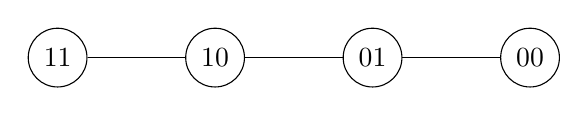
\begin{tikzpicture}
    \node[draw, circle] (A) at (0,0) {11};
    \node[draw, circle] (B) at (2,0) {10};
    \node[draw, circle] (C) at (4,0) {01};
    \node[draw, circle] (D) at (6,0) {00};
    
    \draw (A) -- (B);
    \draw (B) -- (C);
    \draw (C) -- (D);
\end{tikzpicture}
\caption{Representación de los 4 estados}
\label{fig:grafo_4estados_prediccion}
\end{figure}

    \item Una predicción que usa 3 bits de historial, los cuales pasamos a explicar:
        \begin{description}
            \item [Primer bit.] Cuenta con un 1 si se saltó la última vez, 0 si no.
            \item [Segundo bit.] Cuenta con un 1 si se saltó la penúltima vez, 0 si no.
            \item [Tercer bit.] Cuenta con un 1 si se saltó la antepenúltima vez, 0 si no.
        \end{description}
        En caso de haber más unos que ceros, se predica saltar. En caso contrario, se predice no saltar. 

        Este tipo de predicciones se implementan con un registro con desplazamiento.

        Cabe destacar que esta misma predicción puede generalizarse a más bits, siguiente con la misma estrategia. En caso de tener un número par de bits, hay que decidir qué hacer si la cantidad de unos coincide con la cantidad de ceros.
\end{enumerate}
En este tipo de predicciones, para las primeras predicciones (cuando no tenemos un estado prefijado todavía), se realizan predicciones estáticas y luego se puede fijar un estado, en relación a si se saltó o no.

\subsection{Software mejorando el paralelismo}
El software puede mejorar la ejecución de programas, ya que los compiladores pueden realizar cambios sobre el código a ejecutar, antes de traducirlo a lenguaje máquina\footnote{Muchas de estas optimizaciones se describen en la Sesión IV de prácticas.}. Destacamos en esta sección un par de optimizaciones que puede llevar a cabo el software:

\subsubsection{Reordenación de código}
El software puede extraer paralelismo de la aplicación, eliminando dependencias y reduciendo tiempos de penaliación (latencias), lo cual es beneficioso en los procesadores VLIW.

Mostramos el siguiente ejemplo como ilustración de dicha funcionalidad.

\begin{ejemplo}
    Supongamos que queremos ejecutar el Código ensamblador~\ref{cod:ejm7_T4}.
    \begin{listing}[H]
    \begin{minted}[xleftmargin=6cm, linenos]{asm}
add r1, r2, r3
sub r4, r5, r2
cmp r8, r4, r7
jz  r8, 0x2300000F
ld  r2, a
    \end{minted}
    \caption{Código a ejecutar}
    \label{cod:ejm7_T4}
    \end{listing}
    El cual tiene una dependencias de datos tipo RAW entre las líneas 2 y 3, que introducirá tiempos de penalización, al tener que esperar la instrucción 3 a la 2 en la estación de reserva. Sin embargo, el compilador puede darse cuenta de esta dependencia RAW, así como que las instrucciones 1 y 2 no tienen dependencias entre sí, para intercambiar las instrucciones 1 y 2, reduciendo el tiempo de penalización de la instrucción 3 provocada por la dependencia RAW (que no eliminamos pero hacemos que su efecto se vea reducido).
\end{ejemplo}

\subsubsection{Instrucciones de ejecución condicional}
Podemos reducir el número de instrucciones de salto condicional del programa (reduciendo así los riesgos de control), mediante instrucciones de ejecución condicional, como por ejemplo \verb|setxx| o \verb|cmovxx|.

\section{Microarquitectura de ILP VLIW}
Como comentamos en la Sección~\ref{sec:diff_ilp}, los procesadores con paralelismo a nivel de instrucción del tipo VLIW (\emph{Very Long Instruction Word}), sólo son capaces de emitir una instrucción por ciclo, de forma que cada instrucción es capaz de codificar varias operaciones.

Es el compilador quien tiene que realizar todas las labores vistas en este capítulo para una buena planificación en las operaciones.\\

La labor que hacen los compiladores de un procesador VLIW es poner juntas en memoria las operaciones a realizar en cada ciclo de reloj (para que se capten y ejecuten juntas). En caso de disponer de $n$ unidades funcionales para la etapa de ejecución, cada instrucción del procesador VLIW será capaz de ejecutar $n$ operaciones a la vez.\\

La pregunta que nos hacemos ahora es, ¿siempre va a ser posible encontrar $n$ instrucciones independientes (sin dependencias tipo RAW entre ellas) a ejecutar de forma que en cada ciclo queden libres todas las unidades funcionales? la respuesta a esta pregunta es negativa:
\begin{itemize}
    \item O bien no hay $n$ instrucciones consecutivas independientes.
    \item O bien hay una unidad funcional que durante los siguientes $m$ ciclos estará ejecutando una instrucción y no será posible introducir otra del mismo tipo.
\end{itemize}
Cuando algo de esto suceda, se introducirá una operación de no operación (\verb|nop|), relativa a la unidad funcional correspondiente.\\

Cabe destacar que los procesdores VLIW se comercializaron, aunque una de sus grandes contrapartidas es la complejidad que tiene crear un compilador para este tipo de procesadores.
Por otra parte, implementan un cauce mucho más sencillo.
